\section{Illustrative example%: The impossibility of direct reverse engineering generated code
	}
\label{sec:motivation}

We consider a producer-consumer example developed using component-based engineering.
Fig. \ref{fig:cbseexample} (left) shows the component-based model of the example.
The \ttt{p} producer produces data items and sends to a first-in first-out passive communication channel instance \ttt{fifo}.
The latter stores data in order for the consumer to pull it.
The class diagram of \ttt{FIFO} is explored in Fig. \ref{fig:cbseexample} (right).
FIFO persists data items in a sized queue attribute, namely, \ttt{queue}.
The latter is associated with the number of currently stored items (\ttt{numberOfItems}), the capacity (\ttt{MAX\_SIZE}), and other attributes and operations used for validating incoming items and the status of the queue.

The producer's port with \ttt{IPush} as its required interface is connected to the port of FIFO with \ttt{IPush} as its provided interface so that the producer and FIFO can interact with each other through their respective port.
Because FIFO provides two interfaces, it implements these.

The behavior of \ttt{FIFO} is described by using a UML State Machine as in Fig. \ref{fig:fifostatemachine}.
The machine activates the \ttt{Idle} state as initial state.
The latter waits for an item to come to the \ttt{fifo} component (through the \ttt{pPush} port, for instance).
The item is then checked for its validity by using a \ttt{choice} pseudo state.
The \ttt{DataQueuing} state verifies the status of the queue to decide to either add the item to the queue or discard it.  


\begin{figure}
	\centering
	\includegraphics[clip, trim=0cm 14.9cm 14.9cm 0cm, width=\columnwidth]{figures/cbseexample.pdf}
	\caption{Architecture of System (left) and Class diagram of FIFO (right)} 
	\label{fig:cbseexample}
\end{figure}


\begin{figure}
	\centering
	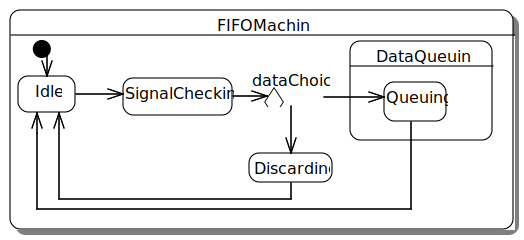
\includegraphics[clip, trim=0.2cm 0cm 0cm 0.1cm, width=1.0\columnwidth]{figures/fifostatemachine.png}
	\caption{FIFO's UML State Machine} 
	\label{fig:fifostatemachine}
\end{figure}

In the next sections, this example will be used for illustrating how XSeparation works.


%\input{sections/statemachinemotivation}

